\documentclass{article} % Changed from assignmeownt to article for standard compatibility
\usepackage{listings}
\usepackage{amsmath}
\usepackage{nccmath}
\usepackage{pdfpages}
\usepackage{graphicx}
\usepackage{caption}
\usepackage{float} % Include the float package for the H specifier


\DeclareMathOperator*{\argmax}{arg\,max}
\DeclareMathOperator*{\argmin}{arg\,min}

\title{Exercise 4}
\author{Tal Grossman, 201512282 , Moshe Yelisevitch, 207423104}
\date{30/07/2024}

\begin{document}
\maketitle

\section{Theory}
\vspace{-1pt} % Adjust this value as needed
For theory sections, please see handwritten solution.
\begin{figure}[H]
    \centering
    \includegraphics[width=0.7\textwidth, page=1]{RL-HW4_Q1_Q2.pdf}
    \caption{Question 1, Page 1}
\end{figure}
\begin{figure}[H]
    \centering
    \includegraphics[width=1.2\textwidth, page=2]{RL-HW4_Q1_Q2.pdf}
    \caption{Question 1, Page 2}
\end{figure}
\begin{figure}[H]
    \centering
    \includegraphics[width=1.2\textwidth, page=3]{RL-HW4_Q1_Q2.pdf}
    \caption{Question 1, Page 3}
\end{figure}
\begin{figure}[H]
    \centering
    \includegraphics[width=1.2\textwidth, page=4]{RL-HW4_Q1_Q2.pdf}
    \caption{Question 1, Page 4}
\end{figure}

\begin{figure}[H]
    \centering
    \includegraphics[width=1.2\textwidth, page=5]{RL-HW4_Q1_Q2.pdf}
    \caption{Question 2, Page 1}
\end{figure}
\begin{figure}[H]
    \centering
    \includegraphics[width=1.2\textwidth, page=6]{RL-HW4_Q1_Q2.pdf}
    \caption{Question 2, Page 2}
\end{figure}

\begin{figure}[H]
    \centering
    \includegraphics[width=1.2\textwidth, page=1]{Hw4Q3.pdf}
    \caption{Question 3, Page 1}
\end{figure}
\begin{figure}[H]
    \centering
    \includegraphics[width=1.2\textwidth, page=2]{Hw4Q3.pdf}
    \caption{Question 3, Page 2}
\end{figure}

\newpage
\section{Programming}

\subsection{Black Jack}
\subsubsection{Item 1 -\textbf{TD(0)}}
completed in python in the attached file \textbf{q1\_TD0.py}
\newline
Ran 300000 episodes with $\alpha = 0.01$ and $\gamma = 0.8$, the results are as follows:
\newline \newline
- Probability of winning: 0.394
\newline
- value for every state: {4: 0.28, 5: 0.26, 6: 0.18, 7: 0.21, 8: 0.48, 9: 0.77, 10: 1.07, 11: 1.19, 12: 0.47, 13: 0.12, 14: 0.04, 15: -0.03, 16: -0.01, 17: -0.2, 18: 0.69, 19: 1.81, 20: 2.99, 21: 4.57}
\subsubsection{Item 1 -\textbf{SARSA}}
completed in python in the attached file \textbf{q1\_SARSA.py}
\newline
    Ran 300000 episodes with $\alpha = 0.01$ and $\gamma = 0.8$, the results are as follows:
\newline \newline
    - The optimal policy is: {4: hit, 5: hit, 6: hit, 7: hit, 8: hit, 9: hit, 10: hit, 11: hit, 12: hit, 13: hit, 14: hit, 15: hit, 16: hit, 17: hit, 18: hit, 19: stand, 20: stand, 21: stand}
\newline
    - Probability of winning with the optimal policy: 0.389
\newline \newline
we can see that the probability of winning is very similar to the one we got with TD(0), which is expected since SARSA is a type of TD(0) algorithm, and the optimal policy is also very similar to the one we got with TD(0).
%In that specific run, it took 263 iterations to converge. The plot of the failure rate is as follows:
%\begin{figure}[H]
%    \centering
%    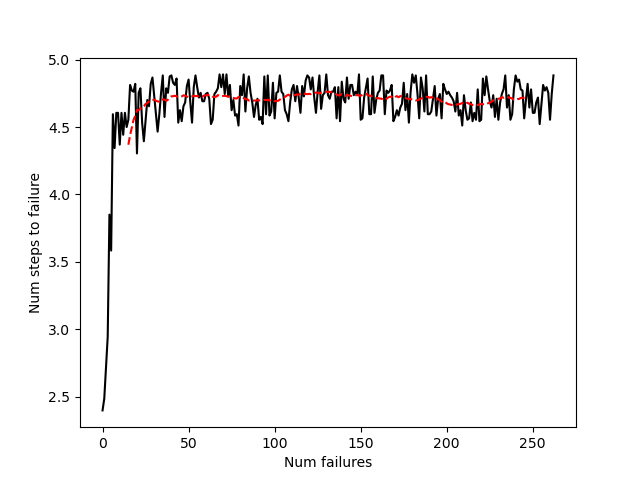
\includegraphics[width=0.7\textwidth]{ex1_263_failure_plot.png}
%\end{figure}
%
%\subsection{Question 2: Q-Learning}
%\subsubsection{Item 1 - tabular\_Q.py}
%The percentage of successful episodes is roughly \text{56.6\%} . The Q-table is as follows:
%\begin{figure}[H]
%\centering
%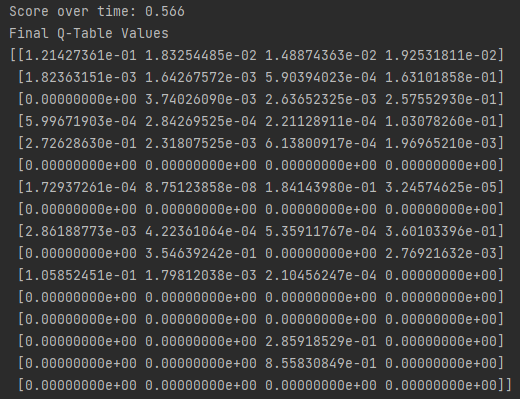
\includegraphics[width=0.6\textwidth]{Q_table_ex2_item1.png}
%\end{figure}
%\subsubsection{Item 2 - network\_Q.py}
%The percentage of successful episodes is roughly \text{34.5\%}.
%This result is worse than what we achieved with tabular Q-learning, probably due to the fact that the network is not
%deep and complicated enough to capture the complexity of the environment. We believe that with a deeper network with
%some activation functions, we could achieve better results.
%
%\begin{figure}[H]
%\centering
%
\includegraphics[width=0.4\textwidth]{score_ex2_item2.png}
%\end{figure}

\end{document}
